\documentclass[
  captions=tableheading,
  bibliography=totoc, 
  titepage=firstiscover,
]{scrartcl}

\usepackage{blindtext} %neuer input

\usepackage{longtable} % Tabellen über mehrere Seiten

\usepackage[utf8]{inputenc} %neuer input

\usepackage{scrhack}

\usepackage[aux]{rerunfilecheck} %Warnung falls nochmal kompiliert werden muss

\usepackage{fontspec} %Fonteinstellungen

\recalctypearea{}

\usepackage[main=ngerman]{babel} %deutsche Spracheinstellung

\usepackage{ragged2e} %neuer input

\usepackage{amsmath, nccmath}

\usepackage{amssymb} %viele mathe Symbole

\usepackage{mathtools} %Erweiterungen für amsmath


\DeclarePairedDelimiter{\abs}{\lvert}{\rvert}
\DeclarePairedDelimiter{\norm}{\lVert}{\rVert}

\DeclarePairedDelimiter{\bra}{\langle}{\rvert}
\DeclarePairedDelimiter{\ket}{\lvert}{\rangle}

\DeclarePairedDelimiterX{\braket}[2]{\langle}{\rangle}{
#1 \delimsize| #2
}

\NewDocumentCommand \dif {m}
{
\mathinner{\symup{d} #1}
}


\usepackage[
  math-style=ISO,
  bold-style=ISO,
  sans-style=italic,
  nabla=upright,
  partial=upright,
  warnings-off={
    mathtools-colon,
    mathtools-overbracket,
  },
]{unicode-math}

\setmathfont{Latin Modern Math}
\setmathfont{XITS Math}[range={scr, bfscr}]
\setmathfont{XITS Math}[range={cal, bfcal}, StylisticSet=1]


\usepackage[
  locale=DE,
  separate-uncertainty=true,
  per-mode=reciprocal,
  output-decimal-marker={,},
]{siunitx}

\usepackage[autostyle]{csquotes} %richtige Anführungszeichen

\usepackage{xfrac}

\usepackage{float}

\floatplacement{figure}{htbp}

\floatplacement{table}{htbp}

\usepackage[ %floats innerhalb einer section halten
  section,   %floats innerhalb er section halten
  below,     %unterhalb der Section aber auf der selben Seite ist ok
]{placeins}

\usepackage[
  labelfont=bf,
  font=small,
  width=0.9\textwidth,
]{caption}

\usepackage{subcaption} %subfigure, subtable, subref

\usepackage{graphicx}

\usepackage{grffile}

\usepackage{booktabs}

\usepackage{microtype} %Verbesserungen am Schriftbild

\usepackage[
backend=biber,
]{biblatex}

\addbibresource{../lit.bib}

\usepackage[ %Hyperlinks im Dokument
  german,
  unicode,
  pdfusetitle,
  pdfcreator={},
  pdfproducer={},
]{hyperref}

\usepackage{bookmark}

\usepackage[shortcuts]{extdash}

%\usepackage{warpcol}


\begin{document}
    \title{V603 Compton-Effekt}
    \author{  
    Tobias Rücker\\
    \texorpdfstring{\href{mailto:tobias.ruecker@tu-dortmund.de}{tobias.ruecker@tu-dortmund.de}}{}}
    
    \date{ Abgabe: 05.05.2020 \vspace{-4ex}}
\maketitle
\thispagestyle{empty}

\newpage
\tableofcontents
\thispagestyle{empty}
\newpage

% Ziel %%%%%%%%%%%%%%%%%%%%%%%%%%%%%%%%%%%%%%%%%%%%%%%%%%%%%%%%%%%%%%%%%%%%%%%%%%%%%%%%%%%%%%%%%%%%%%%%%%%%%%%%%%%%%%%%%%%%%%%%%%%%%%%%%%%%%%%%%%%%%%%%%%%%%%%%%%%%%%%%%%%%%%%%%%%%%%%%%%%%%%%%%%%%%%%%%%%%%%%%%%%%%%%%%

\setcounter{page}{1}
\section{Ziel}\justifying

Der Compton-Effekt stellt in der Physik eine gute Methode dar, um zum Beispiel die Richtung der Herkunft hochenergetischer 
Strahlung zu bestimmen oder um Atome mittels Laser-Kühlung auf tiefe Temperaturen zu bringen. 
Daher wird in einem Experiment die Comptonwellenlänge, zum näheren Verständnis des Compton-Effekts,
mittels der Transmission eines Aluminium-Absorbers bestimmt werden.

% Theorie %%%%%%%%%%%%%%%%%%%%%%%%%%%%%%%%%%%%%%%%%%%%%%%%%%%%%%%%%%%%%%%%%%%%%%%%%%%%%%%%%%%%%%%%%%%%%%%%%%%%%%%%%%%%%%%%%%%%%%%%%%%%%%%%%%%%%%%%%%%%%%%%%%%%%%%%%%%%%%%%%%%%%%%%%%%%%%%%%%%%%%%%%%%%%%%%%%

\section{Theorie}\justifying

% Fehlerrechnung %%%%%%%%%%%%%%%%%%%%%%%%%%%%%%%%%%%%%%%%%%%%%%%%%%%%%%%%%%%%%%%%%%%%%%%%%%%%%%%%%%%%%%%%%%%%%%%%%%%%%%%%%%%%%%%%%%%%%%%%%%%%%%%%%%%%%%%%%%%%%%%%%%%%%%%%%%%%%%%%%%%%%%%%%%%%%%%%%%%%%%%%%%%%%%%%%%%%%%

\section{Fehlerrechnung}\justifying

Für die Berechnung von Messunsicherheiten werden in diesem Protokoll folgende Formeln
verwendet:
\begin{subequations} \label{eq:}
\begin{align} 
\intertext{Zur Bestimmung eines Mittelwertes wird folgende Formel benutzt:
}
    \overline{x} &= \frac{1}{N}\sum_{i=1}^{N} x_i \label{eq:a}
\intertext{Zur Bestimmung der Messunsicherheit bei Mittelwerten wird mit der Formel
}
    \Delta\overline{x} &= \frac{1}{\sqrt{N}} \sqrt{\frac{1}{1-N} \sum_{i=1}^{N} (x_i - \overline{x})^2} \label{eq:b},
\intertext{gearbeitet und die Gaußsche Fehlerfortpflanzung wird mit
}
    \Delta f &= \sqrt{\sum_{i=1}^{N} \left( \frac{\delta f}{\delta x_i} \right)^2 \cdot (\Delta x_i)^2} \label{eq:c}
\intertext{berechnet. Um Ausgleichsgeraden und ihre Parameter zu bestimmen, werden folgende Formeln verwendet:
}
    y &= m \cdot x + b \label{eq:6d} \\ 
    m &= \frac{\overline{xy} - \overline{x} \cdot \overline{y}}{\overline{x^2} - {\overline{x}}^2} \label{eq:e}\\
    b &= \frac{\overline{y} \cdot \overline{x^2} - \overline{xy} \cdot \overline{x}}{\overline{x^2} - {\overline{x}}^2} \label{eq:f}
\end{align}
\end{subequations}
\newpage

% Versuchsaufbau + Versuchsdurchführung %%%%%%%%%%%%%%%%%%%%%%%%%%%%%%%%%%%%%%%%%%%%%%%%%%%%%%%%%%%%%%%%%%%%%%%%%%%%%%%%%%%%%%%%%%%%%%%%%%%%%%%%%%%%%%%%%%%%%%%%%%%%%%%%%%%%%%%%%%%%%%%%%%%%%%%%%%%%%%%%%%%%%%%%%%%%%%%%%%%%%%%%%%%%%%%%%%

\section{Versuchsaufbau und Versuchsdurchführung}\justifying

Zuerst wird der Aufbau für das Emissionspektrum aufgebaut.
Dafür wird in die Röntgenröhre \cite{V603}
\begin{figure}[H]
    \centering
    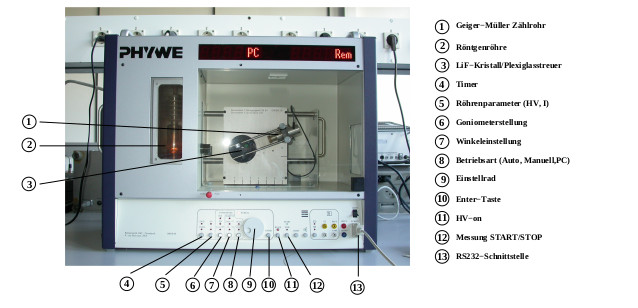
\includegraphics[width=\linewidth]{./images/Aufbau1.jpg}
    \caption{Röntgenröhre}
    \label{fig:1}
\end{figure}
\flushleft{ein\,}\justifying LiF-Kristall sowie eine 2 mm Blende eingebracht. Dann wird auf dem 
Pc über das Programm measure das röntgengerät ausgewählt und
eine Integrationszeit zwischen 5-10s eingestellt. Die Schrittweite wird auf 0,1°
festgelegt und der Winkelbereich wirdso gewählt, dass der gesamte Bremsberg sowie die
charakteristischen Linien enthalten sind. 

\flushleft{Für\,}\justifying die Messung der Comptonwellenlänge wird zuerst die Intensität der Kupferröhre gemessen.
Dafür wird nun eine 5mm Blende statt der 2mm Blende verwendet und der LiF-Kristall
durch einen Plexiglasstreuer ausgetauscht. Das RS232-Kabel wird entfernt und es wird
eine manuelle Messung durchgeführt. Dafür wird der Kristall auf 45° und das Geiger-Müller Zählrohr auf 90°
eingestellt. Danach wird die Intensität der Cu-Röhre gemessen.\\
Zuletzt wird die Intensität mit Aluminium-Absorber in 2 verschiedenen Stellungen bei einer Messzeit von mindestens 300s
 gemessen: \cite{V603}
\begin{figure}
    \centering
    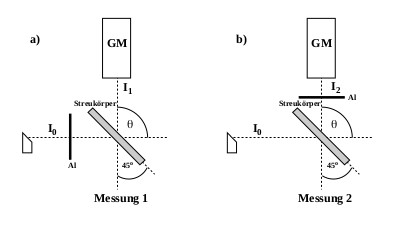
\includegraphics[width=\linewidth]{./images/Aufbau2.jpg}
    \caption{Aufbau der 2 Stellungen}
    \label{fig:2}
\end{figure}
Diese Messung in den 2 Stellungen wird 5 mal wiederholt.

% Auswertung %%%%%%%%%%%%%%%%%%%%%%%%%%%%%%%%%%%%%%%%%%%%%%%%%%%%%%%%%%%%%%%%%%%%%%%%%%%%%%%%%%%%%%%%%%%%%%%%%%%%%%%%%%%%%%%%%%%%%%%%%%%%%%%%%%%%%%%%%%%%%%%%%%%%%%%%%%%%%%%%%%%%%%%%%%%%%%%%%%%%%%%%%%%%%%%%%%

\section{Auswertung}

\begin{table}[H]
    \centering
    \input{table_Cu.tex}
    \caption{Messwerte für das Emissionsspektrum von Kupfer}
    \label{tab:1}
\end{table}


\begin{figure}[H]
    \centering
    \includegraphics[width=\linewidth]{./build/plot_Cu.pdf}
    \caption{Emissionsspektrum von Kupfer}
    \label{fig:a}
\end{figure}





\begin{table}[H]
    \centering
    \input{table_Al.tex}
    \caption{Messwerte für das Transmissionsspektrum von Aluminium}
    \label{tab:2}
\end{table}




\begin{figure}[H]
    \centering
    \includegraphics[width=\linewidth]{./build/plot_T.pdf}
    \caption{Transmission von Aluminium}
    \label{fig:b}
\end{figure}

Die Fitparameter der Geraden
\begin{equation}
T=a \lambda +b
\end{equation}
betragen dabei
\begin{align}
    a = \text{\input{a_Al.tex}}\quad \text{und}\\
    b = \text{\input{b_Al.tex}}.
\end{align}

% Diskussion %%%%%%%%%%%%%%%%%%%%%%%%%%%%%%%%%%%%%%%%%%%%%%%%%%%%%%%%%%%%%%%%%%%%%%%%%%%%%%%%%%%%%%%%%%%%%%%%%%%%%%%%%%%%%%%%%%%%%%%%%%%%%%%%%%%%%%%%%%%%%%%%%%%%%%%%%%%%%%%%%%%%%%%%%%%%%%%%%%%%%%%%%%%%%%%%%%

\section{Diskussion}


% Literatur %%%%%%%%%%%%%%%%%%%%%%%%%%%%%%%%%%%%%%%%%%%%%%%%%%%%%%%%%%%%%%%%%%%%%%%%%%%%%%%%%%%%%%%%%%%%%%%%%%%%%%%%%%%%%%%%%%%%%%%%%%%%%%%%%%%%%%%%%%%%%%%%%%%%%%%%%%%%%%%%%%%%%%%%%%%%%%%%%%%%%%%%%%%%%%%%%%

\newpage
\printbibliography

\end{document}